% !TEX encoding = UTF-8
% !TEX TS-program = pdflatex
% !TEX root = ../tesi.tex
% !TEX spellcheck = it-IT

%**************************************************************
\chapter{Analisi dei Requisiti}
\label{cap:analisi-dei-requisiti}
%**************************************************************

Questo capitolo contiene i requisiti dell'applicazione che sono stati individuati sia discutendo con il tutor aziendale, sia analizzando l'attuale client per iPad di WARDA.

Dal momento che lo scopo dello stage è quello di riprodurre l'applicazione attuale non è stato necessario effettuare un'analisi dei requisiti a partire dai casi d'uso, in quanto i requisiti possono essere estrapolati direttamente dall'applicazione attuale.

Il capitolo inizia quindi con la descrizione delle caratteristiche d'interesse dell'applicazione attuale per poi elencare i requisiti individuati.

%Il contenuto di questo capitolo è il risultato dei vari sprint effettuati, in quanto l'intero processo di sviluppo del prodotto è stato svolto in modo simile a quanto previsto dalla metodologia agile Scrum.

%Dopo un'analisi iniziale dell'applicazione attuale, effettuata in modo da identificare il dominio applicativo, tutte le attività sono state svolte secondo degli \textit{sprint}, ognuno dei quali mirato ad implementare una determinata caratteristica dell'applicazione.

%Ogni \textit{sprint} è stato caratterizzato da un breve riunione con il tutor aziendale, seguita da un'analisi dei nuovi requisiti emersi, per poi passare alla progettazione e all'implementazione delle nuove funzionalità.


\section{Applicazione attuale}

L'applicazione attuale per iPad di WARDA permette di visualizzare il contenuto di una gallery che si trovata sul server principale dell'applicazione.

Oltre alla visualizzazione della gallery è possibile anche creare nuovi asset, recuperando un'immagine dalla libreria interna del dispositivo o dalla fotocamera e accedere alla funzionalità collaborative offerte dalla piattaforma WARDA.

Per il progetto dello stage, l'azienda è interessata solamente alla componente gallery dell'applicazione, in quanto si tratta della parte della applicazione che richiede la maggior quantità di risorse e che attualmente soffre di alcuni problemi prestazionali.

La struttura dati alla base di una gallery realizzata con WARDA è un albero, composto da vari nodi, ognuno dei quali contiene un'insieme di assets e dei possibili filtri.

Per WARDA un'asset è un'immagine a cui vengono associati dei metadati che la descrivono, questi metadati possono poi essere utilizzati per filtrare gli assets presenti in un nodo, in modo da permettere all'utente di visualizzare solamente gli assets con determinate caratteristiche.

\subsection{Pagina di visualizzazione della gallery}

La pagina dell'applicazione che visualizza la gallery è composta da tre parti principali:
\begin{itemize}
\item una lista che visualizza i nodi figli del nodo corrente;
\item una griglia che visualizza gli asset presenti nel nodo corrente;
\item una lista di filtri che visualizza i filtri che possono essere applicati sugli assets contenuti nel nodo corrente.
\end{itemize}
Ognuno di questi componenti sarà descritto nelle seguenti sotto sezioni.

\begin{figure}[htbp]
\centering
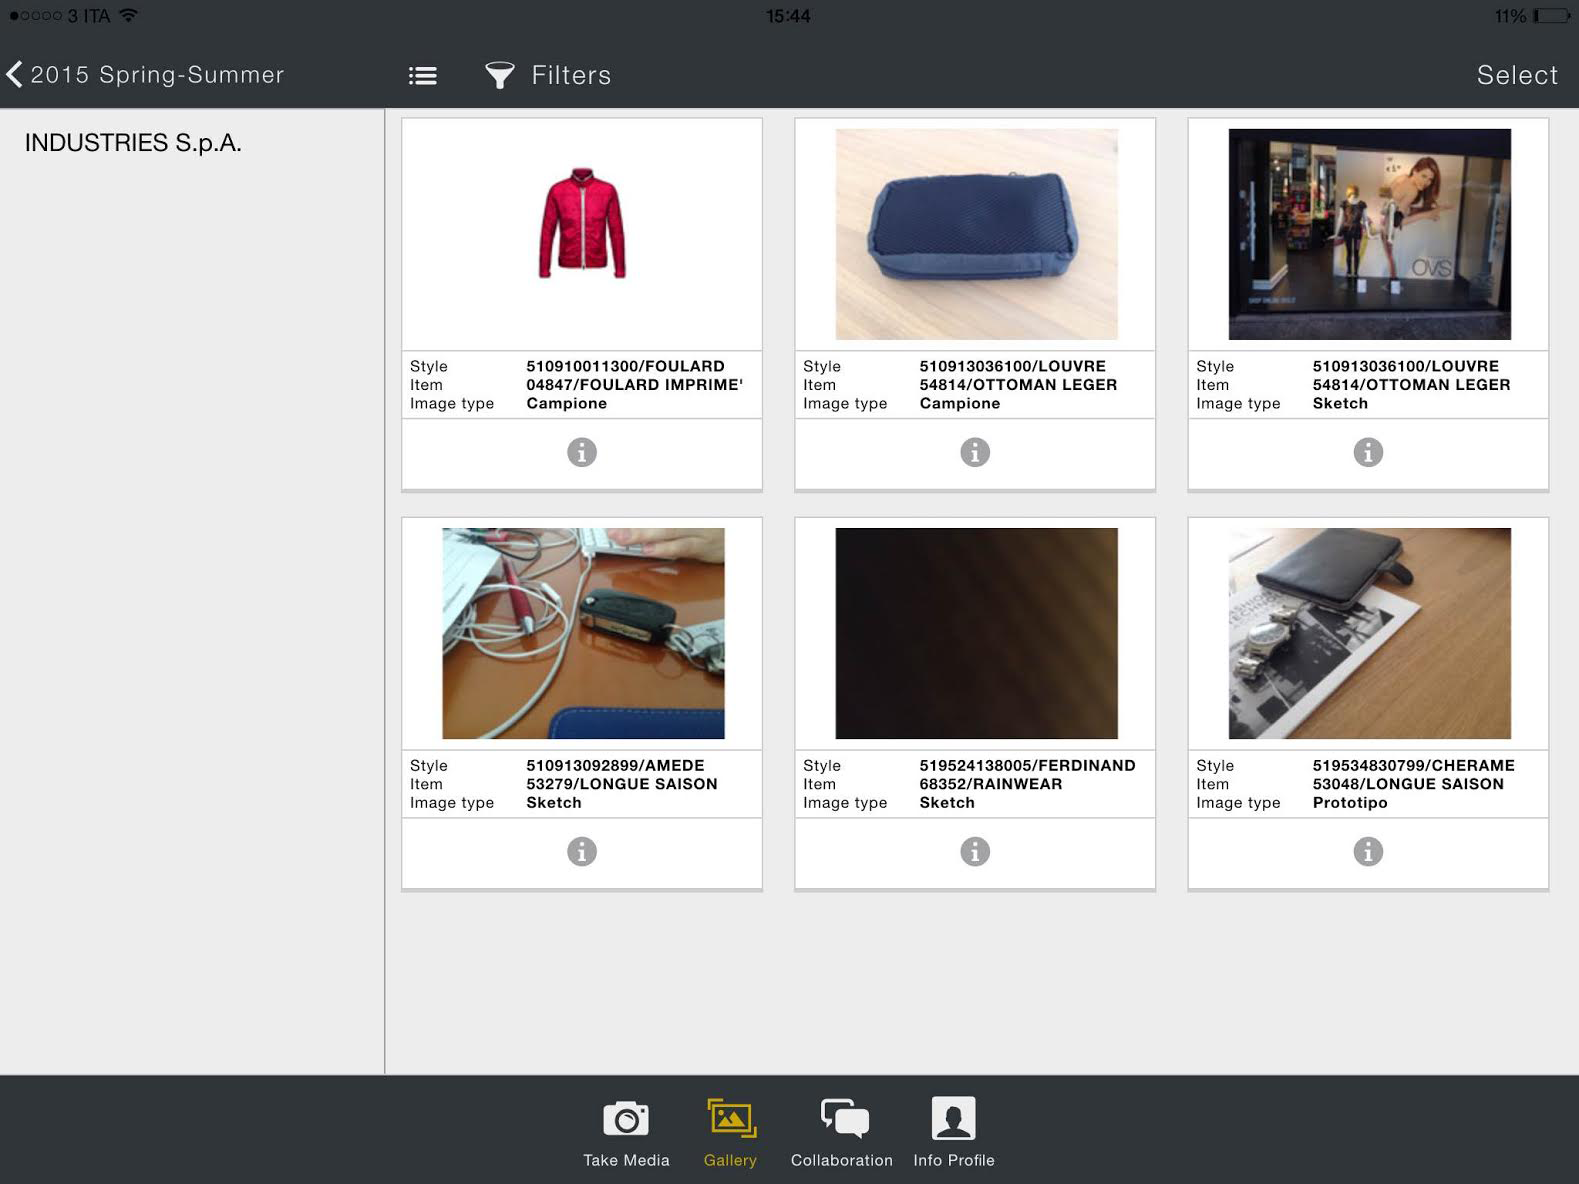
\includegraphics[width=\textwidth]{../immagini/warda-gallery}
\caption{Screenshot della gallery dell'applicazione attuale}  
\end{figure}

\subsubsection{Lista dei nodi}

\begin{figure}[htbp]
\centering
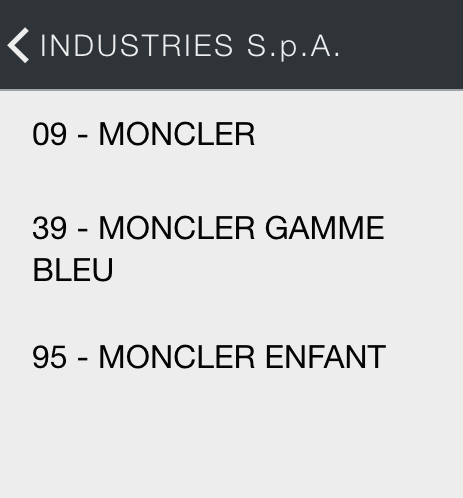
\includegraphics[scale=0.3]{../immagini/warda-gallery-lista-nodi}
\caption{Screenshot della lista dei nodi dell'applicazione attuale}  
\end{figure}

La lista dei figli del nodo corrente visualizza il titolo di ogni nodo e, quando l'utente seleziona un nodo dalla lista, questa viene aggiornata in modo che visualizzi i nodi figli del nodo selezionato. 
La selezione di un nodo dalla lista comporta anche l'aggiornamento della griglia degli assets, la quale andrà a visualizzare gli assets contenuti nel nodo selezionato.

Durante il caricamento dei dati della lista viene visualizzato un indicatore di attività per fornire all'utente un feedback riguardo l'operazione di caricamento dei dati in corso.

Sopra la lista dei nodi è presente un pulsante che permette di tornare al nodo padre del nodo correntemente visualizzato.

Questo pulsante è caratterizzato da una freccia verso sinistra e dal titolo del nodo correntemente visualizzato, nel caso il nodo corrente sia il nodo radice della gallery, il pulsante non deve essere visibile.

\FloatBarrier
\subsubsection{Griglia degli assets}

\begin{figure}[htbp]
\centering
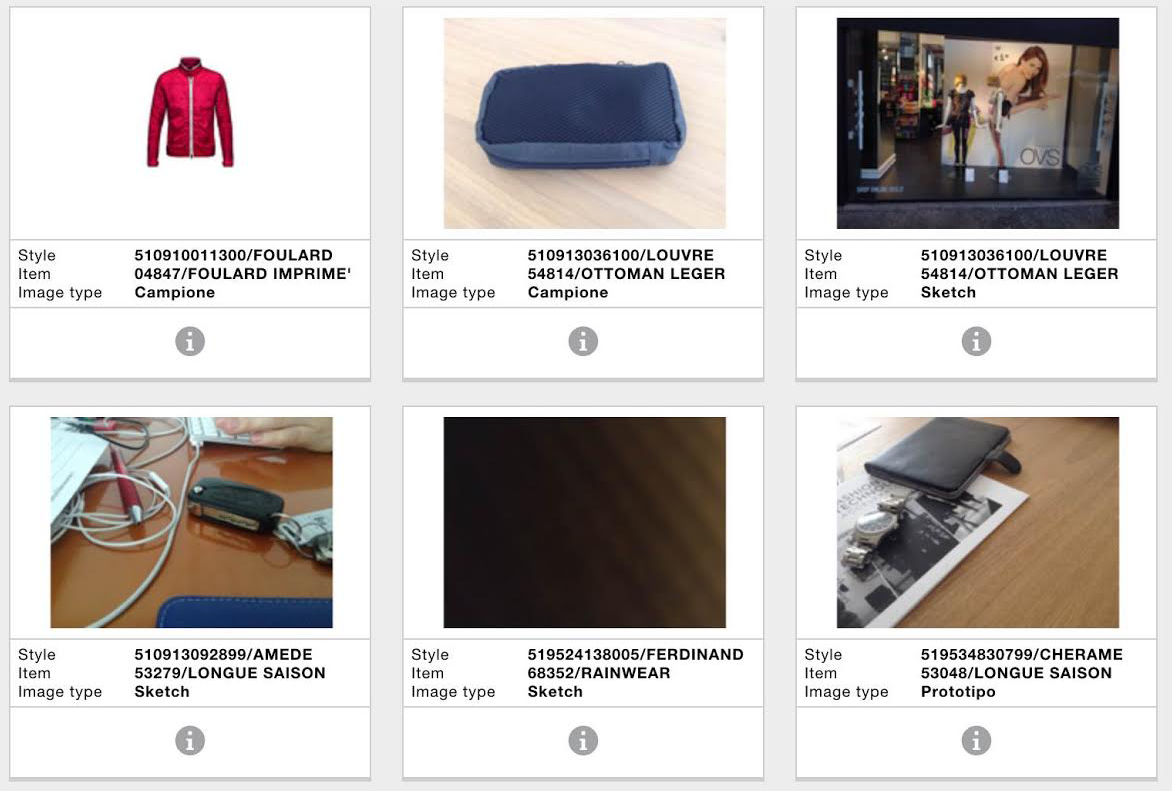
\includegraphics[width=\textwidth]{../immagini/warda-gallery-griglia}
\caption{Dettaglio della griglia degli assets dell'applicazione attuale}  
\end{figure}

La griglia degli assets rappresenta il componente principale dell'applicazione, questa griglia permette di visualizzare, per ogni asset contenuto nel nodo corrente, un'immagine di anteprima e un pulsante che permette all'utente di visualizzare i dettagli dell'asset mediante un \gls{popover}.

\begin{figure}[htbp]
\centering
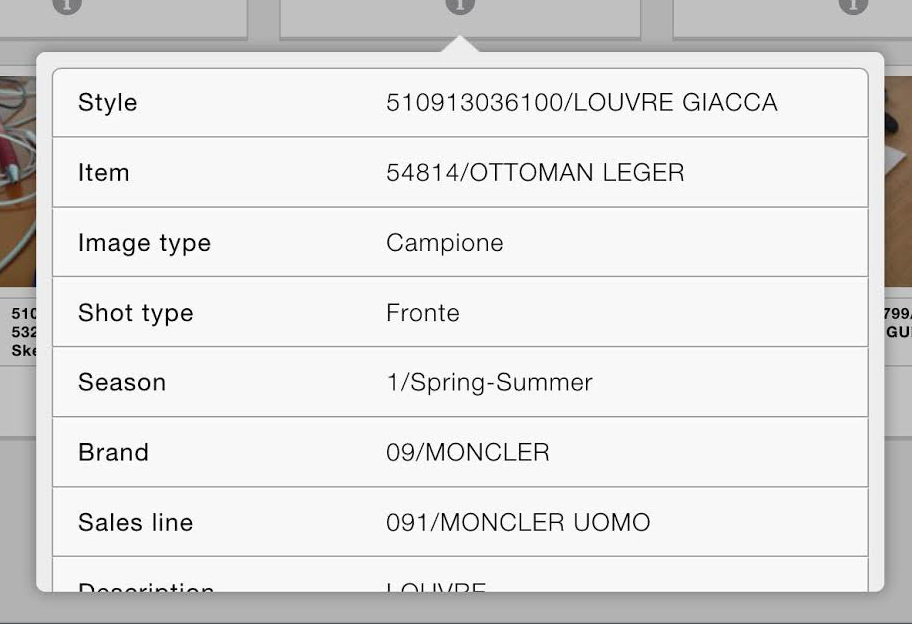
\includegraphics[scale=0.25]{../immagini/warda-gallery-dettaglio}
\caption{Popover che mostra i dettagli di un asset}  
\end{figure}

Se l'utente esegue un \gls{tap} sull'immagine di un asset, viene visualizzata una pagina dell'applicazione contenente i dettagli dell'asset e un'immagine ingrandita, maggiori informazioni riguardo questa pagina sono disponibili nella sezione §\ref{sec:pag-dettaglio-asset}.

Per motivi prestazionali, la griglia non carica subito tutti gli assets contenuti nel nodo corrente ma si limita a visualizzare solo i primi 25 assets, i successivi assets contenuti nel nodo vengono caricati man mano che l'utente prosegue nella visualizzazione della griglia, secondo il sistema dello scroll infinito.

\FloatBarrier
\subsubsection{Lista dei filtri}

\begin{figure}[htbp]
\centering
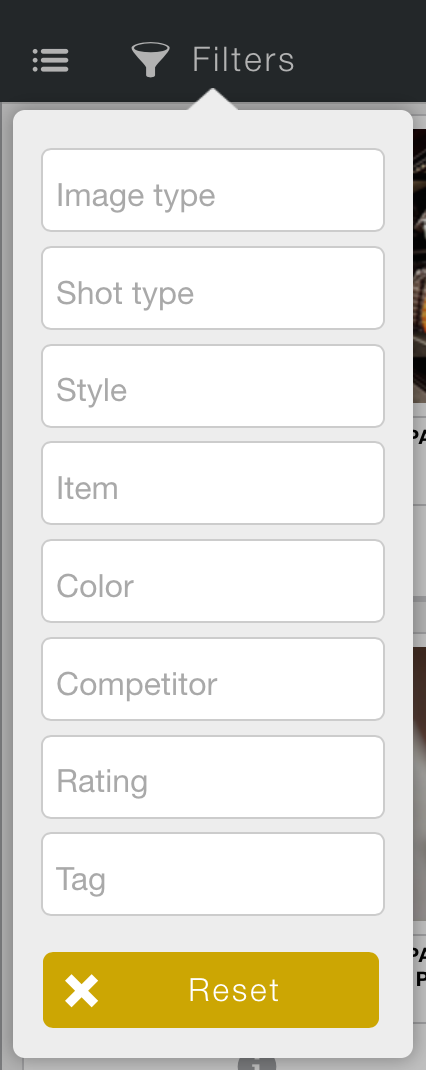
\includegraphics[scale=0.20]{../immagini/warda-filtri}
\caption{Screenshot della lista dei filtri dell'applicazione attuale}  
\end{figure}

La lista dei filtri compare come popover quando l'utente esegue un tap sul pulsante ``Filters'' presente nella barra di navigazione.

Per ogni filtro presente nel nodo corrente, viene visualizzata una lista dei possibili valori che possono essere assegnati al filtro ed una casella di testo che permette all'utente di filtrare i valori presenti nella lista.

\FloatBarrier
\subsection{Pagina di dettaglio di un asset}\label{sec:pag-dettaglio-asset}

Questa pagina contiene l'immagine ingrandita di un asset e una lista con tutti i dettagli dell'asset.

Mediante un apposito pulsante l'utente può nascondere o rendere visibile la lista dei dettagli, in modo da lasciare più spazio all'immagine.

Sull'immagine l'utente può eseguire alcune gesture:
\begin{itemize}
\item \gls{swipe} verso sinistra, per visualizzare l'asset successivo contenuto nel nodo visualizzato dalla gallery;
\item swipe verso destra, per visualizzare l'asset precedente contenuto nel nodo visualizzato dalla gallery;
\item pinch-to-zoom, per ingrandire ulteriormente l'immagine.
\end{itemize}

Infine, nella barra di navigazione della pagina è presente un pulsante che permette all'utente di tornare alla pagina con la visualizzazione a griglia.

\begin{figure}[htp]
\centering
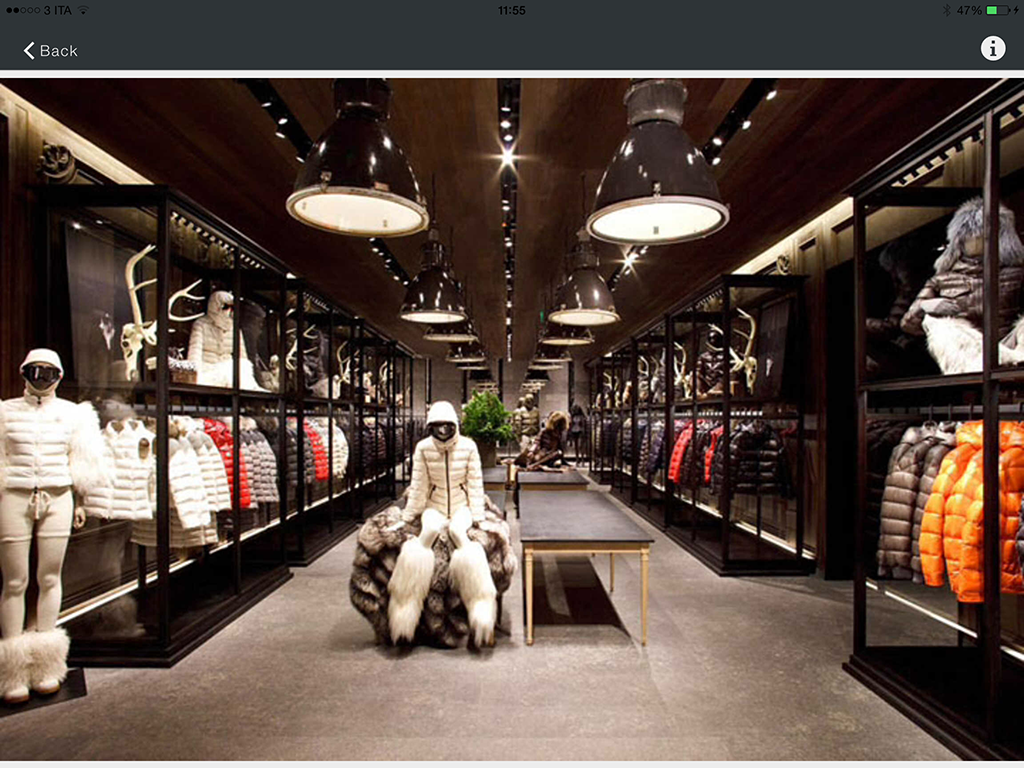
\includegraphics[scale=0.25]{../immagini/warda-asset-no-dettaglio}
\caption{Pagina di dettaglio di un asset}
\end{figure}

\begin{figure}[htp]
\centering
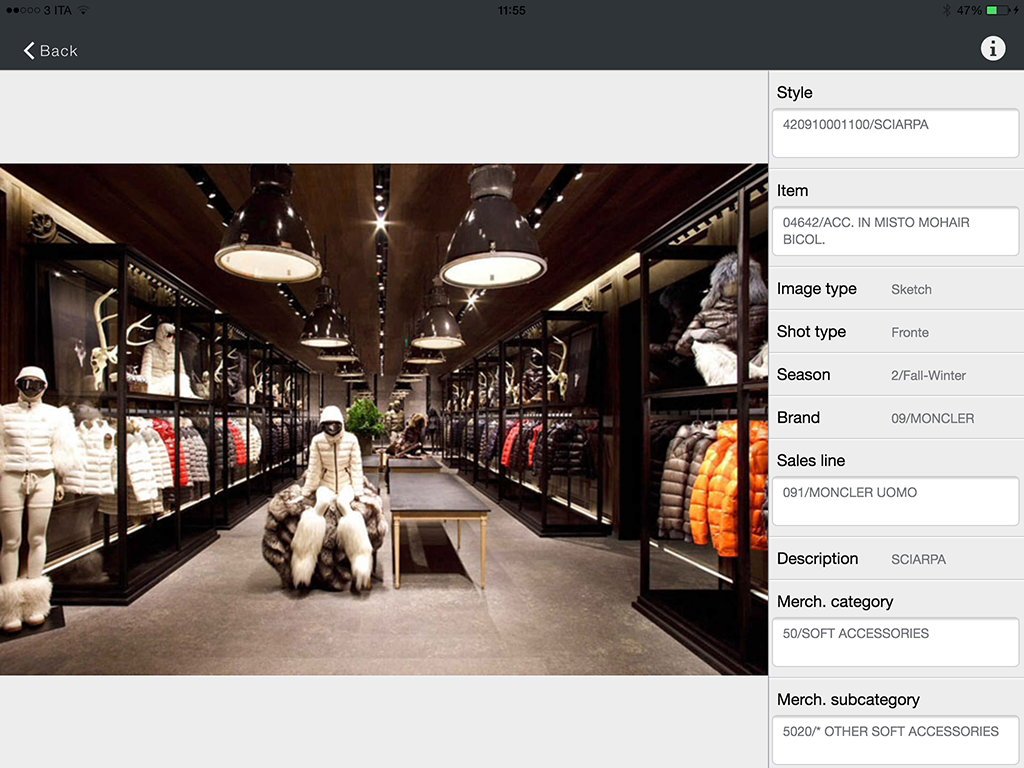
\includegraphics[scale=0.25]{../immagini/warda-asset-dettaglio}
\caption{Pagina di dettaglio di un asset con i dettagli visibili}
\end{figure}
\FloatBarrier
%
%\subsection{Utente tipo}
%L'utente tipo dell'applicazione è una persona che lavora nel mercato della moda e del lusso ed è a conoscenza del funzionamento dei processi di business legati a tale mercato.
%
%Tipicamente l'utente utilizza già il client per desktop di WARDA e vuole utilizzare l'applicazione mobile per consultare velocemente il catalogo degli assets ed eventualmente crearne di nuovi.
%
%Influenzato dall'esperienza con altre applicazioni e dal mondo in cui lavora, l'utente si aspetta che l'applicazione per iPad sia performante e che sia dotata di un interfaccia grafica accattivante e personalizzabile.

\section{Requisiti individuati}

I requisiti individuati dall'analisi dell'applicazione attuale e dalle discussioni con il tutor aziendale sono stati catalogati secondo il codice:
\begin{center}
\textit{R[T][I][C]}
\end{center}
dove:
\begin{itemize}
\item \textbf{T}ipo: specifica la tipologia del requisito e può assumere i seguenti valori:
	\begin{itemize}
	\item \textbf{F} - \textit{funzionale}, cioè che determina una funzionalità dell'applicazione;
	\item \textbf{V} - \textit{vincolo}, che riguarda un vincolo che il prodotto deve rispettare.
	\end{itemize}
\item \textbf{I}mportanza: specifica l'importanza del requisito e può assumere i seguenti valori:
	\begin{itemize}
	\item \textbf{O} - \textit{obbligatorio}, il requisito corrisponde ad un obbiettivo minimo del piano di stage e deve essere soddisfatto per garantire il funzionamento minimo dell'applicazione;
	\item \textbf{D} - \textit{desiderabile}, il requisito corrisponde ad un obbiettivo massimo del piano di stage e deve essere soddisfatto per garantire il funzionamento dell'applicazione;
	\item \textbf{F} - \textit{facoltativo}, indica che il requisito fornisce del valore aggiunto all'applicazione e non era stato previsto nel piano di stage.
	\end{itemize}
\item \textbf{C}odice: rappresenta un codice che identifica il requisito all'interno di una gerarchia. Questo codice è definito in modo che il requisito \textit{RTIx.y} sia un requisito che va a definire con un grado maggiore di dettaglio alcuni degli aspetti del requisito \textit{RTIx}.
\end{itemize}

%subsection
\section{Requisiti}

\subsection{Relazione cliente – fornitore}
Decide molti aspetti del progetto, determinando parte dei bisogni ed imponendo certe scelte sul prodotto. 
Secondo lo standard 12207 vengono riconosciuti come processi primari l'acquisizione e la fornitura. 
L'acquisizione è iniziata dal cliente e richiede adempimenti formali (definizione dei bisogni, gara d'appalto, valutazione e selezione delle offerte..), essa solitamente assegna la responsabilità del progetto ad un solo fornitore. 
La fornitura è un processo che può avere inizio prima o dopo la sigla di un contratto, ed esso richiede diverse attività di tipo PDCA (pianificazione, esecuzione e controllo, revisione e valutazione, consegna e completamento).\\
Si possono fissare diversi tipi di contratti col cliente, i principali sono:
\begin{itemize}
\item \textbf{Contratto a prezzo fisso} dove l'iterazione cliente-fornitore è cruciale per la stima del costo, la definizione e l'accettazione del prodotto, con la possibilità di esonerare il cliente da ogni intervento durante la fase di sviluppo (quindi l'accettazione diventa molto critica);
\item \textbf{Contratto a rimborso dei costi} che prevede frequenti iterazioni cliente-fornitore e si presta bene per attività aperte, prototipali.
\end{itemize}

\subsubsection{L'utente}
L'utente non è necessariamente il cliente, spesso vengono delegate agenzie per l'acquisizione di prodotti per conto di utenti finali, quindi servono più competenze tecniche su aspetti specifici dello sviluppo richiesto.

\subsubsection{Manutenzione}
Una volta che il cliente ha accettato il prodotto, si entra nella fase di sviluppo operativo. 
Questa fase è sotto responsabilità dell'utente e può prevedere o necessitare di un processo di manutenzione.
Tale processo è regolato contrattualmente e l'esecutore della manutenzione può non essere lo stesso del processo di sviluppo (consigliato che le due persone non siano la stessa).

\subsubsection{Organizzazione di un sistema}
Un sistema complesso può essere variamente organizzato e la definizione dell'organizzazione è responsabilità del cliente, con il coinvolgimento dell'utente. 
Il fornitore è chiamato ad aderire all'organizzazione data. La definizione di un sistema è inerentemente gerarchica dove ogni livello propone una relazione cliente-fornitore.
In una visione dall'alto dell'organizzazione a livelli, ciascuna componente di sistema a ciascun livello è il prodotto di uno specifico processo di acquisizione (il fornitore ad un dato livello può necessitare l'acquisizione di uno o più prodotti al livello inferiore)

\subsubsection{Ruoli e responsabilità}
Livello 0 (più alto):
\begin{itemize}
\item \textbf{Cliente} è corresponsabile nella definizione dei bisogni, coadiuvato dall'utente. Ha responsabilità sulla definizione dei vincoli di progetto e dei requisiti (specificati dal fornitore). Esprime accordo con la qualifica di prodotto dichiarata dal fornitore.
\item \textbf{Fornitore} può venire consultato riguardo la definizione dei bisogni e dei vincoli di progetto e concorda con il cliente la specifica dei requisiti da soddisfare. Il fornitore si assume la responsabilità della qualifica e della fornitura del prodotto. Può relazionarsi come cliente con fornitori di livello inferiore.
\end{itemize}

\subsubsection{Relazione tra processi}
Hey! Tu! Si dico a te! Ho bisogno di un'immagine, vedi pagina 14 della fonte.

\subsection{Analisi dei requisiti}
L'attività di analisi prevede di portare ad un accordo tra cliente e fornitore quando le due visioni del problema si incontrano, in modo da identificare il prodotto da commissionare, capire cosa deve essere realizzato e per definire completamente gli accordi committente/fornitore.
Occorre inoltre capire le implicazioni economiche da parte del fornitore (analista) e da parte del cliente c'è solo l'interesse che siano soddisfatti tutti i requisiti, che oltre ad espliciti possono essere impliciti o derivati. 
Da tener presente, dal rapporto Chaos 1995: la prima causa dei fallimenti dei progetti sono i requisiti incompleti.

\subsubsection{Analisi tradizionale e analisi moderna}
L'attività di analisi secondo la prassi di tipo tradizionale prevede uno studio di fattibilità che è lo studio del capitolato d'appalto per una comprensione immediata e per capire se vale la pena entrare nel progetto. Nel caso lo studio di fattibilità dia esito positivo si passa all'analisi dei requisiti che definisce il problema all'interno del dominio, nel quale certi termini, conoscenze devono essere imparate perché sono specifiche del dominio (glossario). 
L'analisi dei requisiti è aiutata dall'uso di linguaggi formali o semi-formali (UML,diagrammi..).\\
Una volta finita l'analisi si passa alla stesura della specifica (progettazione architetturale, spettante al progettista) dove si inizia a trovare la soluzione al problema fornito dall'analista. 
Non è detto che un'analisi dei requisiti abbia una sola soluzione, è compito del progettista trovare la migliore. 
L'enfasi di questa fase è sulla funzionalità e sul modo di ottenere risultati (in base a vincoli).
Dopo la specifica segue la progettazione di dettaglio (top-down) che parte senza avere elementi di soluzione prefissati. Si inizia dal problema, lo si spezza in sottoproblemi e si risolve ogni singola parte. 
Questa fase aggiunge dettaglio agli elementi della soluzione.
\begin{center}
Studio di fattibilità $\rightarrow$ Analisi dei requisiti $\rightarrow$ Specifica $\rightarrow$ Progettazione top-down $\rightarrow$ realizzazione
\end{center}
L'analisi di tipo moderno invece è principalmente orientata agli oggetti (Object Oriented). 
Anch'essa prevede uno studio di fattibilità, un'analisi di tipo orientata agli oggetti che viene supportata da formalismi grafici (es. diagrammi ``use case'') ed ha uno stretto collegamento con la progettazione perché già individua le classi. 
Successivamente all'analisi si ha la progettazione che è sempre di tipo object oriented. 
Essa è coadiuvata dall'utilizzo di componenti prefabbricati e realizza componenti riusabili. 
Dopo la progettazione si ha la programmazione ad oggetti.
\begin{center}
Studio fattibilità $\rightarrow$ Analisi orientata agli oggetti $\rightarrow$ Progettazione OO $\rightarrow$ Programmazione ad oggetti
\end{center}

\subsubsection{Lo studio di fattibilità}
L'obbiettivo principale di questa fase è quello di fornire informazioni necessarie alla decisione sull'effettuazione di un progetto, valutando la fattibilità tecnica ed organizzativa (strumenti, soluzioni architetturali, attrezzature,...).
Tale studio non richiede conoscenze aggiuntive, ma è un'attività molto breve che guarda l'esistente, valutando costi e benefici, individuando i rischi legati alla realizzazione del progetto e considerando le scadenze temporali che il progetto impone. 
Durante tale fase possono emergere delle alternative di tipo architetturale (modello o tipo di sistema da adottare...) o di tipo realizzativo (possibili subappalti).

\subsubsection{Comprensione del dominio}
Consente di acquisire le competenze di dominio per fare una corretta analisi dei requisiti. 
Tali competenze possono essere acquisite tramite la documentazione esistente, oppure tramite la conduzione di interviste agli utenti (clienti) interessati, oppure tramite lo studio di soluzioni esistenti.
Si deve arrivare ad un glossario in cui ci siano tutti (per completezza) e soli (per sinteticità) i termini chiave del dominio. 
Il glossario si può ottenere in 2 modi:
\begin{itemize}
\item mettendo una sezione ``glossario'' in ogni documento;
\item unificare il glossario evolvendolo durante il progetto.
\end{itemize}

\subsubsection{I requisiti}
Si possono dividere in 2 categorie:
\begin{itemize}
\item \textbf{Funzionali}: tradizionalmente i requisiti a cui è dato maggio risalto poiché il prodotto è visto come un insieme di funzionalità.
\item \textbf{Caratteristiche di qualità}: secondo una visione più ampia e moderna legata ad efficienza, affidabilità, secondo modelli della qualità del software e regolata da norme per identificare le caratteristiche di qualità.
\end{itemize}
L'attività di analisi dei requisiti ha come obbiettivo quello di raccogliere i requisiti, redarre il documento Analisi dei Requisiti, valicare i requisiti, rinegoziare i requisiti non chiari o rischiosi, gestire i requisiti.

\subsubsection{Il documento dei requisiti e la sua validazione}
Tradizionalmente i requisiti possono essere estratti da interviste ai clienti/utenti, da questionari scritti, da osservazioni di futuri utenti al lavoro o dallo studio di documenti.
Negli ultimi tempi tale estrazione si è spostata sulla produzione di prototipi o su incontri periodici tra clienti e realizzatori (JAD – Join Application Development).
I requisiti devono poi essere riportati nel ``Documento dei requisiti'' del quale il verificatore si deve accertare di completezza, struttura e correttezza del linguaggio. 
Tale documento non deve fornire una soluzione al problema.
Il documento dei requisiti deve successivamente venire validato controllando la correttezza dell'associazione con l'analisi dei requisiti, indipendentemente dalla forma. Per fare tale validazione si possono usare alcune tecniche:
\begin{itemize}
\item \textbf{Ispezione}: analisi mirata ad alcune parti del prodotto;
\item \textbf{Walkthrough}: analisi esaustiva (completa);
\item \textbf{Matrice delle dipendenze}: legata ai requisiti.
\end{itemize}
Solitamente l'analisi dei requisiti identifica troppi requisiti, quindi serve un negoziato col cliente per modificare la lista dei requisiti individuando quelli obbligatori, quelli desiderabili (non necessari, ma utili) e quelli opzionali.
Tutti i requisiti devono essere classificati e identificabili, quindi dovranno essere registrati in strutture dati apposite e dovranno essere identificati da un numero sequenziale basato sulla struttura del documento. Inoltre occorre anche tenere traccia di eventuali cambiamenti dei requisiti.\\
Il documento di analisi dei requisiti è destinato soprattutto ai progettisti e agli sviluppatori. I prodotti dell'attività di analisi dei requisiti sono spesso documenti scritti in linguaggio naturale con evidente rischio di ambiguità interpretativa. 
Servono quindi alcune linee guida per evitare espressioni ambigue. Esso può contenere quindi un linguaggio di tipo semi-formale (grafici, diagrammi) o di tipo formale.\\
La struttura di tale documento prevede un'introduzione che spiega lo scopo del documento, del prodotto, eventuali definizioni, acronimi e riferimenti. Ci sarà poi una descrizione generale del progetto che specifica il contesto del prodotto, le sue funzioni, le caratteristiche dell'utente utilizzatore ed eventuali vincoli o limiti del prodotto.\\
Sarà anche presente un glossario per i termini non di uso comune, quelli specifici del dominio del prodotto. 
Ovviamente si avrà la lista dei requisiti che specificherà quelli funzionali, quelli di qualità e di interfaccia. 
Sarà anche definito l'ambiente di esecuzione del sistema e se necessario i vincoli sul formato dei dati.
Si può inoltre prevedere un appendice e un indice (molto utile).

\subsection{Dai requisiti al progetto architetturale}
Definizione: Un requisito è una proprietà (attributo) che occorre possedere per soddisfare un determinato bisogno.\\
Le attività primarie richieste sono:
\begin{itemize}
\item \textbf{Analisi dei bisogni}: serve a definire dei requisiti a livello di sistema (a responsabilità del cliente) e
di specificare dei requisiti software;
\item \textbf{Partizionamento del sistema in componenti}: decomposizione del problema in parti di sistema;
\item \textbf{Attribuzione dei requisiti ai componenti}: ogni componente soddisfa qualche requisito.
\end{itemize}
L'unione dei componenti dà l'architettura.

\subsubsection{Classificazione dei requisiti}
Occorre distinguere tra attributi di prodotto ed attributi di processo:
Gli \textbf{attributi di prodotto} definiscono le caratteristiche richieste al sistema da sviluppare (esempio: specifica di una funzione da calcolare). Esprimono requisiti funzionali determinando le capacità computazionale richieste al sistema e requisiti non funzionali riducendo i gradi di libertà disponibili nella definizione della soluzione.

Gli \textbf{attributi di processo} pongono vincoli sulla conduzione e sulle uscite delle attività previste dal processo.
Esempio: imposizione di una particolare tecnologia di sviluppo (un linguaggio, uno strumento).

Tutti i requisiti devono essere verificabili poiché chi impone un requisito deve sapere come accertarne il soddisfacimento e chi è chiamato a soddisfare un requisito deve poterne stimare il costo di verifica.
Alcuni requisiti derivano implicitamente da attributi di prodotto e/o di processo assegnati dal cliente o decisi dal fornitore

\begin{center}
\textbf{IMMAGINE!!!}
Schema della classificazione dei requisiti
\end{center}

Alcuni requisiti di primo livello (di sistema) possono non essere soddisfacibili perché possono essere:
\begin{itemize}
\item Tecnicamente impossibili (ad esempio integrare parti software scritte in linguaggi incompatibili tra loro);
\item Possibili, ma di implementazione troppo costosa (come considerare un componente senza possederne i sorgenti);
\item Possibili, ma mutuamente esclusivi tra loro (come usare componenti standard e avere un limite sul sistema).
\end{itemize}
L'analisi dei requisiti deve accertare la soddisfacibilità dei requisiti rispetto ai vincoli esistenti sui processi del progetto. 
Al termine dell'analisi i requisiti confermati devono essere tutti necessari e sufficienti: nessun bisogno trascurato e nessuna caratteristica superflua. 
Una priorità relativa può essere assegnata ai requisiti confermati.

\subsubsubsection{Progettazione architetturale}
Essa segue l'attività di analisi e può essere influenzata da esigenze od opportunità di riuso (meglio se sistematico) di componenti che possono essere di tipo aziendale, commerciale o imposte dal cliente. 
Le componenti riusabili che possono includere codice sorgente od eseguibile, specifiche di interfaccia, modelli architetturali.

\subsubsection{L'ingegneria dei requisiti}
\textbf{Ingegneria dei requisiti}: termine che denota l'insieme delle attività necessarie per il trattamento sistematico dei requisiti. 
I requisiti software sono uno dei prodotti del relativo processo.

L'ingegneria dei requisiti deve essere vista come un ciclo PDCA: da formalizzare e pianificare (modello di processo, piano di attività), da eseguire e gestire (responsabilità primarie, organizzative, di supporto), da verificare e migliorare (a livello di efficienza di processo e di qualità del prodotto).

Tutto ciò richiede responsabilità con competenze di ingegneria del processo.
Si possono inoltre individuare altre attività e competenze richieste dal processo (già visti):
\begin{itemize}
\item \textbf{Analisi dei requisiti}: analisi delle fonti, classificazione, modellazione concettuale, decomposizione del sistema, allocazione, negoziazione;
\item \textbf{Verifica e validazione}: tramite revisione interna e/o esterna, prototipazione, analisi del modello concettuale;
\item \textbf{Produzione (dei documenti di specifica)}: Studio di Fattibilità, Analisi dei Requisiti, Specifica Tecnica;
\item \textbf{Gestione e manutenzione dei prodotti}: tracciamento delle attribuzioni, gestione dei cambiamenti.
\end{itemize}

Tecniche di analisi delle fonti:
\begin{itemize}
\item Interviste con il cliente;
\item Generazione ed analisi di scenari - Prototipazione che può essere: interna (per il fornitore) oppure esterna (per il cliente);
\item Discussioni creative ``Brainstorming'' (approccio maieutico);
\item Osservazione dei comportamenti e dei bisogni.
\end{itemize}
Definizioni:\\
\textbf{Verifica}: intende accertare che l'esecuzione di un dato processo non abbia introdotto errori. è principalmente rivolta al processo, ma applica anche ai prodotti di processi intermedi. 
\begin{center}
$\rightarrow$ \textit{Did I build the system right?}
\end{center}
\textbf{Validazione}: intende accertare che l'uscita dell'insieme di processi eseguiti sia il prodotto atteso.
\begin{center}
 $\rightarrow$ \textit{Did I build the right system?}
\end{center}

\section{Riepilogo requisiti}

In totale sono stati individuati 52 requisiti, ripartiti tra le varie tipologie secondo quanto riportato nelle seguenti tabelle.
\\ \\ \\
\begin{minipage}{\textwidth}
  \begin{minipage}[b]{0.49\textwidth}
    \centering
      \begin{tabular}{|l|c|} \hline
      \textbf{Importanza} & \textbf{\#} \\ \hline
  Obbligatori & 29 \\ \hline
  Desiderabili & 12 \\ \hline
  Facoltativi & 11 \\ \hline
  Totale & 52 \\ \hline
\end{tabular}
      \captionof{table}{Numero di requisiti per importanza}
	\end{minipage}
	  \hfill
  \begin{minipage}[b]{0.49\textwidth}
    \centering
         \begin{tabular}{|l|c|} \hline
      \textbf{Tipologia} & \textbf{\#} \\ \hline
  Funzionali & 48 \\ \hline
  Vincolo & 4 \\ \hline
    Totale & 52 \\ \hline
\end{tabular}
    \captionof{table}{Numero di requisiti per tipologia}
  \end{minipage}
\end{minipage}
 \\ \\ \\

\begin{minipage}{\textwidth}
  \begin{minipage}[b]{0.49\textwidth}
    \centering
    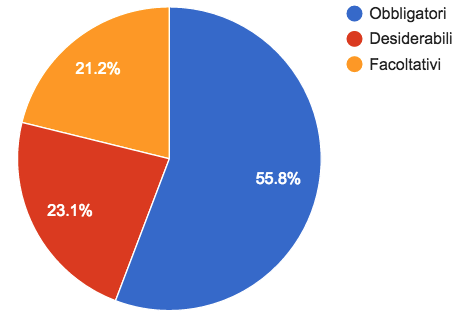
\includegraphics[scale=0.7]{../immagini/requisiti-totale-importanza}
      \captionof{figure}{Requisiti per importanza}
	\end{minipage}
	  \hfill
  \begin{minipage}[b]{0.49\textwidth}
    \centering
  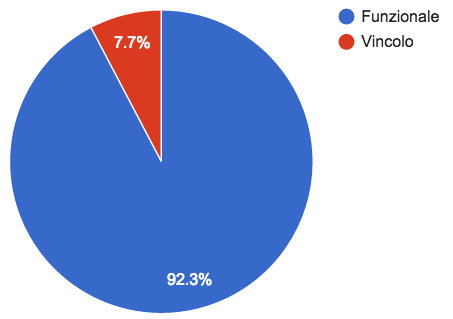
\includegraphics[scale=0.7]{../immagini/requisiti-totale-tipologia}
      \captionof{figure}{Requisiti per tipologia}
  \end{minipage}
\end{minipage}



